
\begin{enumerate}

\item A car has two wipers which do not overlap. Each wiper has a blade of length $21 \mathrm{cm}$ sweeping through an angle of $120\degree$. Find the total area cleaned at each sweep of the two blades.

\item Sides $AB$ and $BC$ and median $AD$ of a triangle $ABC$ are respectively proportional to sides $PQ$ and $QR$ and median $PM$ of $\triangle PQR$.Show that $\triangle ABC \sim \triangle PQR$.

\item Through the mid-point $M$ of the side $CD$ of a parallelogram $ABCD$,the line $BM$ is drawn intersecting $AC$ in $L$ and $AD$ (produced) in $E$.Prove that $EL = 2BL$. 

\item In the given figure, $O$ is the center of the circle .$AB$ and $AC$ are tangents drawn to the circle from point $A$. If $\angle BAC = 65\degree $, then find the measure of $\angle BOC $.
	\begin{figure}[!ht]
		\centering
		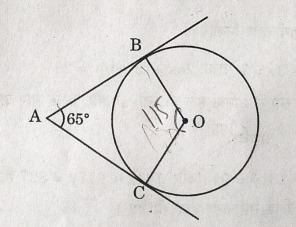
\includegraphics[width=\columnwidth]{figs/last5.jpg}
		\caption{}
		\label{fig:enter-label}
	\end{figure}

\newpage
\item In the given figure, $O$ is the centre of the circle and $QPR$ is a tangent to it at $P$.Prove that $\angle QAP + \angle APR = 90\degree$.

	\begin{figure}[!ht]
		\centering
		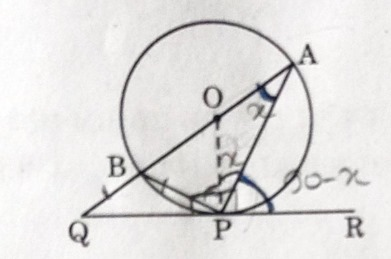
\includegraphics[width=\columnwidth]{figs/last4.jpg}
		\caption{}
		\label{fig:enter-label}
	\end{figure}
\newpage
\item In an annual day function of a school, the organizers wanted to give a cash prize along with a memento to their best students.Each memento is made as shown in the figure and its base $ABCD$ is shown from the front side.The rate of silver plating \rupee~20 $per  \mathrm{cm}^2$.

	\begin{figure}[!ht]
		\centering
		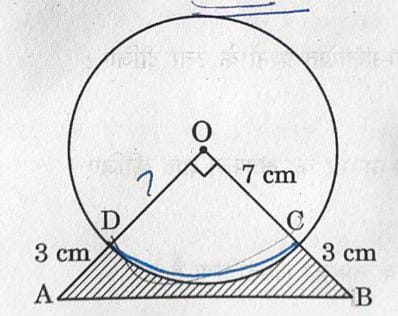
\includegraphics[width=\columnwidth]{figs/last3.jpg}
		\caption{}
		\label{fig:enter-label}
	\end{figure}

	\text Based on the above, answer the following question:
		\begin{enumerate}
			\item What is the area of the quadrant $ODOC$?
			\item Find the area of $\triangle AOB$.
			\item
			\begin{enumerate}
				\item What is the total cost of silver plating the shaded part $ABCD$?
				\item What is the length of arc $CD$ ?
			\end{enumerate}
		\end{enumerate}
\newpage
\item In a coffee shop, coffee is served in two types of cups.One is cylindrical  in shape with diameter $7 \mathrm{cm}$ and height $14 \mathrm{cm} $ and the other is hemispherical with diameter $21 \mathrm{cm}$.

	
	\begin{figure}[!ht]
		\centering
		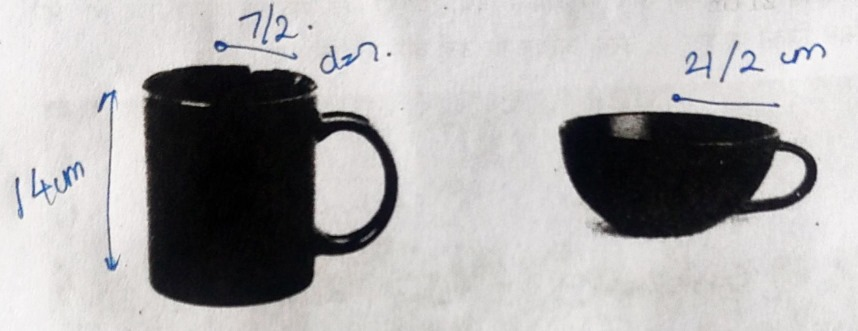
\includegraphics[width=\columnwidth]{figs/last2.jpg}
		\caption{}
		\label{fig:enter-label}
	\end{figure}

	\text Based on the above, answer the following question:
	\begin{enumerate}
		\item  Find the area of the cylindrical cup.
		\item
		\begin{enumerate}
			\item  What is the capacity of the hemispherical cup?
			\item Find the capacity of the cylindrical cup.
		\end{enumerate}
		\item   What is the curved surface area of the cylindrical cup?
         \end{enumerate}

\newpage	
\item Show that the points $\brak{-2,3}, \brak{8,3}$ and $\brak{6,7} $ are the vertices of a right-angled triangle.

\item If $Q\brak{0,1}$ is equidistant from $P\brak{5,-3}$ and $R\brak{x,6}$,find the values of $x$.


\end{enumerate}

